\documentclass[10pt,aspectratio=169]{beamer}
\usetheme{metropolis}
\usepackage{amsmath, amssymb}
\usepackage{tikz}
\usetikzlibrary{arrows.meta, positioning, shapes.geometric}
\usepackage{booktabs}

\definecolor{LayerD}{HTML}{3B6EA5}
\definecolor{LayerS}{HTML}{3B8A5A}
\definecolor{LayerR}{HTML}{A5343B}

\setbeamertemplate{frametitle continuation}{}
\metroset{block=fill}

\title{Fragmented Housing Regulation as a\\ Fiscal-Federalism Breakdown}
\subtitle{A new measure of discretionary review, and the leakage of state preemption}
\author{Daniel Posthumus}
\date{June 2026}

\begin{document}

\maketitle

% ---------------------------------------------------------------- 2
\begin{frame}{The question, and what is new}
California has spent a decade preempting local zoning (SB\,9/10, the builder's remedy). Yet
the lever localities actually pull --- \textbf{discretionary review} --- is left untouched and
goes \emph{unmeasured}.

\bigskip
\textbf{The contribution.} I build the first item-level dataset of the discretionary margin from
planning-commission minutes, and use it to ask:
\begin{enumerate}
  \item[\textcolor{LayerR}{Q2}] \textbf{What is the leakage of preemption?} When the state forces
  open \emph{one} regulatory margin, do jurisdictions reassert restriction through the margin it
  leaves untouched? \emph{Does preemption loosen supply, or get clawed back?}
  \item[\textcolor{LayerR}{Q1}] \textbf{How large is the distortion from fragmentation?} The gap
  between decentralized, non-internalized regulation and a regional planner who internalizes the
  spillover --- \emph{how much housing is ``missing,'' at what welfare cost?}
\end{enumerate}

\medskip
\footnotesize Q2 is reduced-form and rests on the new data; Q1 layers a structural model on top.
The order reflects what I am surest of.
\end{frame}

% ---------------------------------------------------------------- 3
\begin{frame}{The key object: restriction on \emph{two} margins}
A jurisdiction restricts supply by lowering the by-right envelope \emph{or} raising the
discretionary friction. The literature measures only the first.
\medskip
\begin{columns}[T]
\begin{column}{0.5\textwidth}
\begin{block}{By-right envelope $\bar z_j$}
The zoning map: what a project obtains \emph{ministerially}, no hearing.
\begin{itemize}\small
  \item What LLM zoning measurement \textbf{sees} (Gupta \& Barik; Bartik 2024).
  \item What preemption \textbf{targets}.
\end{itemize}
\end{block}
\end{column}
\begin{column}{0.5\textwidth}
\begin{alertblock}{Discretionary tax $\tau_j$ \quad(\emph{my data})}
The review friction on projects exceeding $\bar z_j$: process exposure, mobilized opposition,
approval-with-conditions, continuances, rare denial.
\begin{itemize}\small
  \item What code-based measures \textbf{cannot} see.
  \item What preemption \textbf{leaves untouched}.
\end{itemize}
\end{alertblock}
\end{column}
\end{columns}
\medskip
\[ \text{Effective restriction}\quad r_j = g(\bar z_j,\tau_j),\qquad
   \text{lower } \bar z_j \ \textbf{or}\ \text{raise } \tau_j. \]
\footnotesize Council sets the slow map $\bar z_j$; the planning commission sets the fast
$\tau_j$. \textbf{Their substitutability drives both questions} --- and the binary approve/reject
vote, which shows little variation in the minutes, misses it entirely.
\end{frame}

% ---------------------------------------------------------------- 4
\begin{frame}{Measuring $\tau_j$: from minutes to data}
\textbf{Source.} Planning-commission meeting minutes, parsed item-by-item via an LLM/NLP
pipeline into a structured panel.
\medskip
\begin{columns}[T]
\begin{column}{0.46\textwidth}
\textbf{Extracted per agenda item}
\begin{itemize}\small
  \item Request type \& project scale
  \item Stance-marked speaker counts (support / oppose)
  \item Outcome: approve, \textbf{approve-with-conditions}, continuance, denial
  \item \# and type of conditions imposed
  \item Hearing exposure (continuances, re-hearings)
\end{itemize}
\end{column}
\begin{column}{0.54\textwidth}
\begin{block}{Why this is the friction, not the vote}
Denials are rare; restriction shows up as \emph{conditions, delay, and exposure} that deter
applications before they reach a vote. $\tau_j$ aggregates these into a jurisdiction-level
discretionary cost.
\end{block}
\footnotesize \emph{Validation:} hand-coded subsample for precision/recall; cross-check $\tau_j$
against permit timelines and approval lags where available.
\end{column}
\end{columns}
\medskip
\footnotesize\emph{(Backup: one fully coded meeting item, raw text $\to$ extracted fields.)}
\end{frame}

% ---------------------------------------------------------------- 5
\begin{frame}{Preemption and its leakage (Q2)}
Preemption (ministerial mandates, by-right upzoning, the builder's remedy) raises the cost of a
tight \emph{envelope} $\bar z_j$ --- but not of the \emph{discretionary} tax $\tau_j$.
\medskip
\begin{block}{Leakage}
With $r_j=g(\bar z_j,\tau_j)$ and the two margins substitutes, a preemption that loosens
$\bar z_j$ induces a still-restriction-demanding jurisdiction to \textbf{raise} $\tau_j$ in
compensation (more conditions, more opposition entertained, more continuances). Effective
restriction falls by \emph{less} than the envelope change implies; \textbf{the conditional
approval rate need not move at all}.
\[ \text{Leakage } \in [0,1]:\quad 0=\text{preemption fully effective},\ \ 1=\text{fully clawed back}. \]
\end{block}
\textbf{Identification.} SB\,9/10 and builder's-remedy episodes are shocks to $\bar z_j$; I trace
the $\tau_j$ response in the minutes around each episode. \emph{This is the cleanest test in the
project --- a real shock, a directly measured response.}
\end{frame}

% ---------------------------------------------------------------- 6
\begin{frame}{Why it is a \emph{federalism} question: the spillover}
\begin{columns}[T]
\begin{column}{0.56\textwidth}
Regulation is set by jurisdictions ($J\!\approx\!109$ in the Bay Area) far \textbf{finer} than the
housing submarkets ($S\!\ll\!J$) and the \emph{one} regional labor market they sit in.
\medskip

A worker earns the regional wage $w_m=w(N)$, $w'>0$ (agglomeration). So:
\begin{itemize}
  \item the \textbf{benefit} of access-providing housing is \emph{regional}
  (submarket price relief + higher $w_m$);
  \item the \textbf{cost} of that density is \emph{local} disamenity.
\end{itemize}
\medskip
A jurisdiction bears the full local disamenity of an approval but captures little price relief
--- most \emph{leaks} to co-submarket neighbors. It under-supplies and \textbf{free-rides}.
\end{column}
\begin{column}{0.44\textwidth}
\begin{block}{Submarket price (the externality)}
\[ p_{s} \;=\; \frac{\alpha\, N_{s}}{H_{s}}, \qquad H_s=\!\!\sum_{j:\,s(j)=s}\!\!H_j \]
Housing built in \emph{any} $j\in s$ lowers the price faced by incumbents in \emph{every}
$j\in s$.
\end{block}
\begin{exampleblock}{The Oates wedge (Q1)}
Decentralized Nash regulation is \emph{tighter} than the internalized optimum --- and the gap
grows as $j$ becomes atomistic within its submarket.
\end{exampleblock}
\end{column}
\end{columns}
\end{frame}

% ---------------------------------------------------------------- 7
\begin{frame}{The framework: three layers, one equilibrium}
\centering
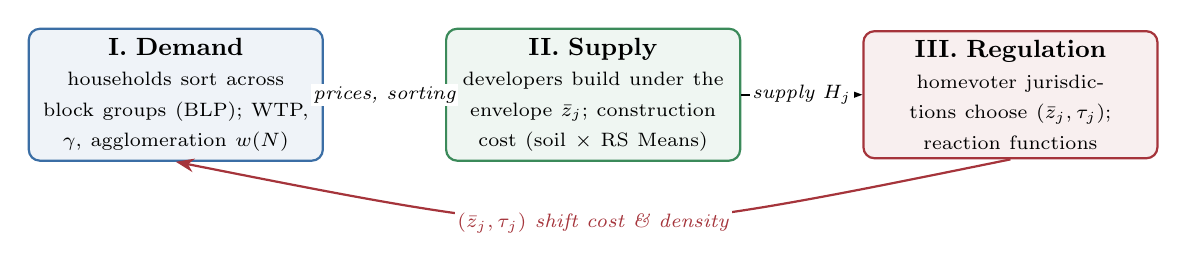
\begin{tikzpicture}[
  font=\small,
  boxbase/.style={rounded corners, draw, thick, text width=3.5cm, align=center,
              minimum height=1.5cm},
  boxD/.style={boxbase, fill=LayerD!8, draw=LayerD},
  boxS/.style={boxbase, fill=LayerS!8, draw=LayerS},
  boxR/.style={boxbase, fill=LayerR!8, draw=LayerR},
  lab/.style={midway, font=\scriptsize\itshape, fill=white, inner sep=1pt},
  >={Stealth[]}]
\node[boxD] (D) at (0,0) {\textbf{I. Demand}\\ \scriptsize households sort across
  block groups (BLP); WTP, $\gamma$, agglomeration $w(N)$};
\node[boxS] (S) at (5.3,0) {\textbf{II. Supply}\\ \scriptsize developers build under the
  envelope $\bar z_j$; construction cost (soil $\times$ RS Means)};
\node[boxR] (R) at (10.6,0) {\textbf{III. Regulation}\\ \scriptsize homevoter
  jurisdictions choose $(\bar z_j,\tau_j)$; reaction functions};
\draw[->, thick] (D) -- node[lab]{prices, sorting} (S);
\draw[->, thick] (S) -- node[lab]{supply $H_j$} (R);
\draw[->, thick, LayerR] (R.south) .. controls (5.3,-1.9) .. node[lab]{$(\bar z_j,\tau_j)$ shift cost \& density} (D.south);
\end{tikzpicture}
\vspace{0.6em}
\begin{itemize}\small
  \item \textbf{Layers I--II} (demand \& supply) recover the primitives needed to value any
  counterfactual allocation: who lives where, willingness to pay, how supply responds.
  \item \textbf{Layer III} (the \emph{market for regulation}) is where the federalism breakdown
  lives, and where Q1 is posed.
\end{itemize}
\end{frame}

% ---------------------------------------------------------------- 8
\begin{frame}{The reaction function (Q1)}
Because $p_{s(j)}$ depends on neighbors' regulation, Layer III is a \textbf{game}:
\[ \big(\bar z_j,\tau_j\big) = R_j\big(\bar z_{-j},\tau_{-j}\big),\qquad
   -j = \text{co-submarket neighbors only}. \]
\begin{itemize}
  \item A neighbor \emph{loosens} $\Rightarrow$ submarket price falls $\Rightarrow$ a
  homevoter-pivotal $j$ \emph{tightens}: regulation is \textbf{strategically substitutable}.
\end{itemize}
\begin{block}{What the slope buys}
Under the Decentralization Theorem's efficient case (no spillovers), jurisdictions need not
respond to one another. A robustly \emph{nonzero} slope, once confounders are ruled out, is
the spillover made visible --- its sign and magnitude quantify how badly the Oates condition
fails.
\end{block}
\footnotesize $\Rightarrow$ requires a \textbf{multi-jurisdiction panel}; a single metro cannot,
even in principle, reveal a reaction function.
\end{frame}

% ---------------------------------------------------------------- 9
\begin{frame}{Identification: the open problem I most want your read on}
We see only \emph{equilibrium} regulation, not the objective that generated it. Recovering
$(\phi_j\lambda_j,\ g(\cdot),\ \text{demand}+w(N))$ is what licenses the counterfactuals.
\medskip
\begin{columns}[T]
\begin{column}{0.5\textwidth}
\textbf{The threat to $R_j$:} a nonzero slope is consistent with
\begin{itemize}\small
  \item the \textbf{spillover} (the mechanism), \emph{but also}
  \item yardstick competition, or common submarket shocks (Brueckner 1998, 2003).
\end{itemize}
Separating these is the crux --- and where I would most value your guidance.
\end{column}
\begin{column}{0.5\textwidth}
\textbf{Leverage I have:}
\begin{itemize}\small
  \item \textbf{Soil cost-shifter} (SSURGO foundation cost $\times$ RS Means), residualized
  against seismic / slope / open-space capitalization.
  \item \textbf{Preemption episodes} (SB\,9/10, builder's remedy) as shocks to $\bar z_j$ that
  trace the $\tau_j$ response.
  \item \textbf{Submarket-size variation} in the free-riding wedge
  ($\partial p_s/\partial \text{supply}_j=-p_s/H_s$); BLP instruments for prices.
\end{itemize}
\end{column}
\end{columns}
\vspace{0.3em}
{\footnotesize\emph{Routing:} soil/topography is standard supply-side identification (Saiz). The
strategic-interaction step is structural IO.}
\end{frame}

% ---------------------------------------------------------------- 10
\begin{frame}{Data --- demand side built, regulation side is the contribution}
\begin{columns}[T]
\begin{column}{0.5\textwidth}
\textbf{Regulation (Layer III) --- novel}
\begin{itemize}\small
  \item \textbf{Discretionary margin $\tau_j$:} item-level dataset from planning-commission
  minutes via LLM/NLP. \alert{Invisible to code-based measures.}
  \item \textbf{By-right margin $\bar z_j$:} Gupta \& Barik / Bartik LLM zoning --- \emph{your
  pointer}. I lean on theirs for $\bar z_j$; my data is the $\tau_j$ margin they can't see.
\end{itemize}
\end{column}
\begin{column}{0.5\textwidth}
\textbf{Demand \& supply (Layers I--II) --- assembled}
\begin{itemize}\small
  \item CoreLogic/Cotality \textbf{5.3M transactions} (price spine, geocoded to block group).
  \item ACS PUMS+tables, \textbf{LODES} job access ($w(N)$), TIGER + BG$\leftrightarrow$jurisdiction
  crosswalk.
  \item Amenities (open space, transit, schools), \textbf{crime} (SF/Oakland incident + FBI
  county), IRS migration.
  \item \textbf{SSURGO soil} cost-shifter instrument (BG-level).
\end{itemize}
\footnotesize $\sim$1.5\,GB, fully documented (16-pp provenance + diagnostics report).
\end{column}
\end{columns}
\end{frame}

% ---------------------------------------------------------------- 11
\begin{frame}{Where I am}
\textbf{Surest:} the $\tau_j$ data and the leakage test (Q2) --- new measure, real preemption
shocks, directly observed response.

\smallskip
\textbf{Most uncertain:} identifying the reaction-function slope (Q1) against yardstick
competition and common shocks; and the soil-cost exclusion restriction.

\bigskip
\begin{enumerate}
  \item Does the leakage result stand on its own as a first paper, with Q1 as the structural
  extension --- or would you sequence it differently?
  \item On $R_j$: is there variation you would trust to separate spillover from common shocks?
  \item Is the soil cost-shifter excludable from sorting after the controls, in your view?
  \item Practically --- what would you do first?
\end{enumerate}
\end{frame}

\end{document}